\documentclass[twoside]{article}
\author{Michele Mazza}
% Pacchetti di Codifica e Lingua
\usepackage[utf8]{inputenc}
\usepackage[T1]{fontenc}
\usepackage[italian]{babel}

% Pacchetti Grafici e Diagrammi
\usepackage{graphicx}
\usepackage{tikz}
\usepackage{tikz-3dplot}
\usetikzlibrary{angles,quotes,arrows.meta, positioning, 3d, matrix, calc}
\usepackage{pgfplots}
\pgfplotsset{compat=1.18}

% Pacchetti Matematici
\usepackage{amsmath, amssymb}

% Scegliere tra amsthm e ntheorem
%\usepackage{ntheorem}
% Se si preferisce amsthm, commentare la riga sopra e decommentare la seguente
\usepackage{amsthm}
\usepackage{cancel}

% Pacchetti per Tabelle e Unità di Misura
\usepackage{geometry}
\usepackage{siunitx}
\usepackage{booktabs}
\usepackage{tabularx}
\usepackage{colortbl}
\usepackage{adjustbox}

% Pacchetti per Layout e Formattazione
\usepackage{fancyhdr}
\usepackage{float}
\usepackage{microtype}
\usepackage{multicol}

% Altri Pacchetti Utili
\usepackage{mdframed}
\usepackage{animate}
\usepackage{ulem}
\usepackage{eurosym}

% Pacchetto enumitem
\usepackage{enumitem}

% Definizioni dei Colori e Comandi Personalizzati
\definecolor{lightblue}{HTML}{9cd8fc}
\definecolor{myblue}{HTML}{139FE9}
\definecolor{myblack}{HTML}{303030}
\definecolor{mygray}{HTML}{787878}
\definecolor{mywhite}{HTML}{c7c7c7}
\newcommand{\norm}[1]{\left\lVert#1\right\rVert}

% Ambienti Personalizzati
% Usa \theoremstyle e \theorembodyfont come necessario
\newmdtheoremenv[
    backgroundcolor=orange!10,
    linecolor=myblue,
    linewidth=0pt,
    leftmargin=0pt,
    rightmargin=0pt,
    innerleftmargin=10pt,
    innerrightmargin=10pt,
    innertopmargin=10pt,
    innerbottommargin=10pt,
    nobreak
]{curiosity}{Curiosità}

\newmdtheoremenv[
    font=\normalfont\small,
    linewidth=0pt,
    innerleftmargin=10pt,
    innerrightmargin=10pt,
]{example}{Esempio}

\newmdtheoremenv[
  backgroundcolor=lightblue,
  linecolor=myblue,
  linewidth=1.5pt,
  innertopmargin=10pt,
  innerbottommargin=10pt,
  innerrightmargin=10pt,
  innerleftmargin=10pt,
  nobreak
]{theorem}{Teorema}

\newmdtheoremenv[
  backgroundcolor=gray!10,
  linewidth=0pt,
  innertopmargin=-5pt,
  innerbottommargin=5pt,
  innerrightmargin=10pt,
  innerleftmargin=10pt,
  nobreak
]{definition}{Definizione}

\newmdtheoremenv[
  backgroundcolor=gray!10,
  linecolor=myblue,
  linewidth=1.5pt,
  innertopmargin=-5pt,
  innerbottommargin=5pt,
  innerrightmargin=10pt,
  innerleftmargin=10pt,
  nobreak
]{proposition}{Proposizione}


% Configurazioni di fancyhdr
\pagestyle{fancy}
\fancyhf{}
\fancyhead[RE,RO]{\nouppercase{\rightmark}}
\fancyfoot[C]{\thepage}
\renewcommand{\headrulewidth}{0.0pt}
\renewcommand{\footrulewidth}{0pt}
\geometry{a4paper, left=20mm, right=20mm, top=20mm, bottom=20mm}

\usepackage{titlesec} % Pacchetto per personalizzare i titoli delle sezioni

% Definisci i colori per le diverse sezioni
\titleformat{\section}
{\color{black}\normalfont\Large\bfseries}
{\thesection}{1em}{}

\titleformat{\subsection}
{\color{red}\normalfont\large\bfseries}
{\thesubsection}{1em}{}

\titleformat{\subsubsection}
{\color{blue}\normalfont\normalsize\bfseries}
{\thesubsubsection}{1em}{}

% Pacchetti Aggiuntivi
\usepackage{xparse,array}

% Pacchetto Hyperref (inserito per ultimo)
\usepackage{hyperref}

\begin{document}
\title{Fondamenti di Chimica}
\maketitle
\hrulefill
\section{Indicazioni corso}
Prova scritta di 2 h.\\
Voglio migliorare il voto?\\
30 minuti ti fa vedere la prova e capisci se la puoi migliorare.\\
Ti ritiri conservi la vecchia prova.\\
Se consegni sostituisci il vecchio.\\
Caricano compito fac-simile su virtuale.\\
\section{Struttura atomica della materia e sue proprietà}
\subsection{Classificazione della materia}
\begin{figure}[H]
  \centering
  \begin{tikzpicture}[node distance=4cm]
    \tikzstyle{box} = [rectangle, draw,minimum width=3cm, minimum height=1cm, text centered, thick]
    \node (Materia) [box] {Materia};
    \node (FisEt) [box, below left of=Materia] {Sistemi fisicamente eterogenei};
    \node (FisOm) [box, below right of=Materia] {Sistemi fisicamente omogenei};
    \node (ChimEt) [box, below left of=FisOm] {Sistemi chimicamente eterogenei};
    \node (ChimOm) [box, below right of=FisOm] {Sistemi chimicamente omogenei};
    \node (Elem) [box, below right of=ChimOm] {Elementi};
    \node (Com) [box, below left of=ChimOm] {Composti};
    \draw [-stealth, thick] (Materia) -- (FisEt);
    \draw [-stealth, thick] (Materia) -- (FisOm);
    \draw [-stealth, thick] (FisOm) -- (ChimEt);
    \draw [-stealth, thick] (FisOm) -- (ChimOm);
    \draw [-stealth, thick] (ChimOm) -- (Elem);
    \draw [-stealth, thick] (ChimOm) -- (Com);
  \end{tikzpicture}
\end{figure}
\textbf{Elementi} : Sono formati da atomi tutti uguali, si trovano nella Tavola Periodica.\\
\noindent
\textbf{Composti} : Sono formati da atomi diversi, hanno composizione fissa.\\
\subsection{Struttura atomica}
\subsubsection{Teoria atomica}
\begin{figure}[H]
  \centering
  \begin{tikzpicture}[node distance=1.5cm]
    \tikzstyle{box} = [rectangle, draw,minimum width=3cm, minimum height=1cm, text centered, thick]
    \node (Fil1) [box] {Democrito(468-370 a.C.)};
    \node (Fil2) [box, below of = Fil1] {Epicuro(341-270 a.C.)};
    \node (Fil3) [box, below of = Fil2] {Lucrezio(96-11 a.C.)};
    \node (Fis1) [box, below of = Fil3, fill = myblue] {Dalton(1808)};
    \draw [-stealth, thick] (Fil1) -- (Fil2);
    \draw [-stealth, thick] (Fil2) -- (Fil3);
    \draw [-stealth, thick] (Fil3) -- (Fis1);
    \draw[-, thick] (Fis1) -- ++(0,-1);
  \end{tikzpicture}
\end{figure}
\begin{multicols}{2}
  \begin{enumerate}
    \item La materia è costituita da atomi indivisibili e indistruttibili - (\textbf{Falsa} Esistono gli isotopi che decadono)
    \item Tutti gli atomi di uno stesso elemento hanno la stessa massa e le stesse proprietà chimiche - (\textbf{Falso} Isotopi stesso elemento, diversa massa) - (\textbf{Vero} stesse proprietà chimiche)
    \item Atomi di elementi diversi hanno masse diverse e proprietà chimiche diverse (\textbf{Vero})
    \item Gli atomi di elementi diversi si combinano fra loro in rapporti di numeri interi e generalmente piccoli dando origine a composti (\textbf{Vero})
  \end{enumerate}
  \columnbreak
  \begin{figure}[H]
    \centering
    \begin{adjustbox}{valign=center}
      
\includegraphics[width=0.2\textwidth]{src/image-001.pdf}
    \end{adjustbox}
  \end{figure}
\end{multicols}
\begin{figure}[H]
  \centering
  \begin{tikzpicture}[node distance=1.5cm]
    \tikzstyle{box} = [rectangle, draw,minimum width=3cm, minimum height=1cm, text centered, thick]
    \node (Fis1) [box, fill = myblue] {Thomson(1906)};
    \draw[-, thick] (Fis1) -- ++(0,-1);
    \draw[-stealth, thick] (0,+1) -- ++(Fis1);
  \end{tikzpicture}
\end{figure}
\begin{multicols}{2}
  \begin{enumerate}
    \item Da esperimenti con raggi catodici, scopre l'elettrone
    \item L'atomo è neutro quindi deve esistere una carica positiva(Protone)
    \item Modello a panettone
  \end{enumerate}
  \columnbreak
  \begin{figure}[H]
    \centering
    \begin{adjustbox}{valign=center}
      
\includegraphics[width=0.2\textwidth]{src/image-002.pdf}
    \end{adjustbox}
  \end{figure}
\end{multicols}
\begin{figure}[H]
  \centering
  \begin{tikzpicture}[node distance=1.5cm]
    \tikzstyle{box} = [rectangle, draw,minimum width=3cm, minimum height=1cm, text centered, thick]
    \node (Fis1) [box, fill = myblue] {Rutherford(1908)};
    \draw[-, thick] (Fis1) -- ++(0,-1);
    \draw[-stealth, thick] (0,+1) -- ++(Fis1);
  \end{tikzpicture}
\end{figure}
\begin{multicols}{2}
  \begin{enumerate}
    \item Scopre il nucleo atomico
    \item Nucleo contenente protoni e neutroni, elettroni in orbita
    \item Modello planetario
  \end{enumerate}
  \columnbreak
  \begin{figure}[H]
    \centering
    \begin{adjustbox}{valign=center}
      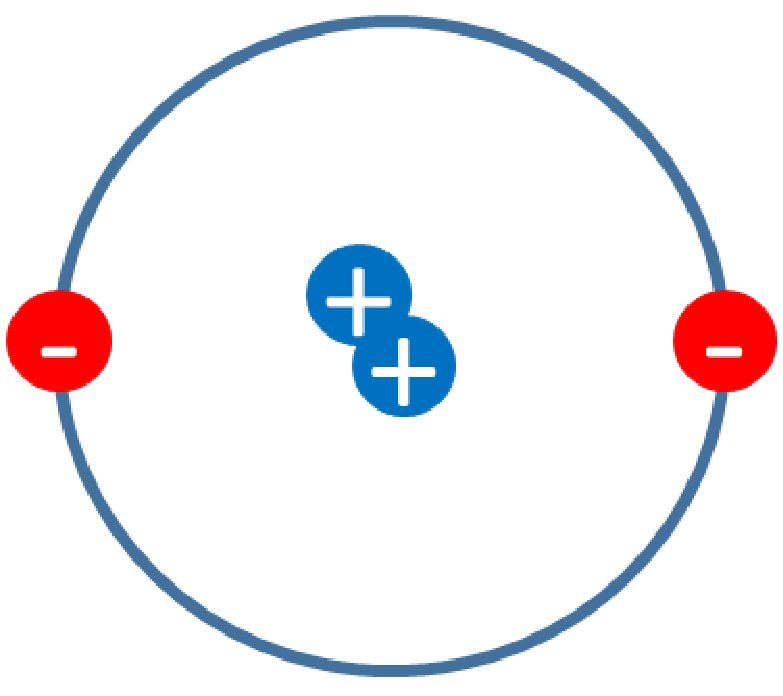
\includegraphics[width=0.2\textwidth]{src/image-003.pdf}
    \end{adjustbox}
  \end{figure}
\end{multicols}
\subsubsection{Le particelle fondamentali}
\begin{table}[H]
  \centering
  \begin{tabular}{|c|c|c|c|c|c|}
    \hline
    \rowcolor{myblue}
    \textbf{Particella} & \textbf{Simbolo} & \multicolumn{2}{|c|}{\textbf{Massa}} & \multicolumn{2}{|c|}{\textbf{Carica}  }                                      \\
    \hline
                        &                  & SI \(\left[g\right]\)                & atomica                                 & SI \(\left[C\right]\)    & atomica \\
    Elettrone           & \(e^-\)          & \(9.11 \times 10^{-31}\)             & \(0.0005\)                              & \(-1.6 \times 10^{-19}\) & \(-1\)  \\
    Protone             & \(p^+\)          & \(1.67 \times 10^{-27}\)             & \(1\)                                   & \(1.6 \times 10^{-19}\)  & \(1\)   \\
    Neutrone            & \(n^0\)          & \(1.67 \times 10^{-27}\)             & \(1\)                                   & \(0\)                    & \(0\)   \\
    \hline
  \end{tabular}
\end{table}
\noindent
\textbf{Unità di carica atomica} : \(1\ \text{uca} = 1.6 \times 10^{-19} \text{C}\)\\
\textbf{Unità di massa atomica} : \(1\ \text{uma} = 1.67 \times 10^{-27} \text{kg}\)\footnotemark[1]\\
\footnotetext[1]{La massa atomica è definita come la dodicesima parte della massa di un atomo di carbonio-12}
\subsubsection{La struttura dell'atomo}
\begin{figure}[H]
  \centering
  \begin{tikzpicture}[node distance=2cm]
    \tikzstyle{box} = [rectangle, draw,minimum width=1.5cm, minimum height=1.5cm, text centered, thick]
    \node (El) [box, fill = green, font=\huge] {$^{A}_{Z}$X};
    \node (Es) [box, fill = green, font=\huge, right of = El] {$^{14}_{7}$N};
    \draw [-stealth, thick] (El) -- (Es);
  \end{tikzpicture}
\end{figure}
\paragraph[short]{Numero atomico (Z)} numero di protoni nel nucleo (o anche elettroni se l'atomo è neutro)
\begin{equation}
  \boxed{Z = \text{numero di elettroni} \quad \lor \quad Z = \text{numero di protoni}}
\end{equation}
Atomi con \(Z\) uguali appartengono allo stesso elemento chimico, hanno le stesse proprietà \textbf{chimiche}.
\paragraph[short]{Numero di massa (A)} numero di protoni e neutroni nel nucleo
\begin{equation}
  \boxed{A = Z + N}
\end{equation}
corrisponde al numero di \textbf{nucleoni} (particelle nel nucleo)
\paragraph[short]{Carica nucleare (+Z)}
numero di protoni nel nucleo
\paragraph[short]{Numero di neutroni (N)}
\begin{equation}
  \boxed{N = A - Z}
\end{equation}
\begin{center}
  \small
  \begin{minipage}{0.7\textwidth}
    \textcolor{violet}{\uline{\textbf{Esempio quiz}}}:\\
    \begin{figure}[H]
      \centering
      \begin{tikzpicture}[node distance=1.5cm]
        \tikzstyle{box} = [rectangle, draw,minimum width=1cm, minimum height=1cm, text centered, thick]
        \node (El) [box, fill = green, font=\large] {$^{12}_{6}$C};
      \end{tikzpicture}
    \end{figure}
    \(^{12}_{6}C\) quanti protoni, neutroni, elettroni?\\
    \(A = 12\)\\
    \(Z = 6\)\\
    \(N = 12 - 6 = 6\)\\
    \(p^+ = 6\)\\
    \(n^0 = 6\)\\
    \(e^- = 6\)\\
  \end{minipage}
\end{center}
\paragraph[short]{Nuclide}
Ogni singola specie nucleare individuata da un numero atomico (\(Z\)) e da un numero di massa (\(A\)).
\begin{figure}[H]
  \centering
  \begin{tikzpicture}[node distance=1.5cm]
    \tikzstyle{box} = [rectangle, draw,minimum width=1cm, minimum height=1cm, text centered, thick]
    \node (El1) [box, fill = green, font=\large] {$^{A}_{Z}$X};
  \end{tikzpicture}
\end{figure}
\paragraph[short]{Isotopi}
Nuclidi di uno stesso elemento chimico aventi lo stesso numero atomico(\(Z\)) ma diverso numero di massa(\(A\)).
\begin{figure}[H]
  \centering
  \begin{tikzpicture}[node distance=1.5cm]
    \tikzstyle{box} = [rectangle, draw,minimum width=1cm, minimum height=1cm, text centered, thick]
    \node (El1) [box, fill = green, font=\large] {$_{6}$C};
    \node (El2) [font=\large, left of = El] {$^{12}$C};
    \node (El3) [font=\large, below left of = El] {$^{13}$C};
    \node (El4) [font=\large, below of = El] {$^{14}$C};
    \draw [-stealth, thick] (El2) -- (El1);
    \draw [-stealth, thick] (El3) -- (El1);
    \draw [-stealth, thick] (El4) -- (El1);
  \end{tikzpicture}
\end{figure}
\paragraph[short]{Ioni}
Atomi o molecole che hanno perso o guadagnato elettroni.
\begin{itemize}
  \item \textbf{Cationi} : hanno perso elettroni, Na$^+$
  \item \textbf{Anioni} : hanno guadagnato elettroni, O$^{2-}$
\end{itemize}

\subsubsection{Massa atomica}
\paragraph[short]{Massa atomica assoluta}
si misura con la spettrometria di massa
\begin{equation}
  \boxed{m = \text{massa di un atomo}}
\end{equation}
\paragraph[short]{Unità di massa atomica}
\begin{equation}
  \boxed{1\ \text{uma} = \frac{1}{12} \text{massa di un atomo di }^{12}_{6}C}
\end{equation}
\paragraph[short]{Massa atomica relativa}
\begin{equation}
  m_{i} = \frac{m}{1\ \text{uma}}
\end{equation}
in natura gli atomi di un elemento non hanno tutti la stessa massa, la massa atomica relativa è la media ponderata delle masse atomiche dei vari isotopi.
\begin{equation}
  \boxed{M_{r} = \frac{\sum_{i}^{n} m_i \cdot f_i}{\sum_{i}^{n} f_i}}
\end{equation}
dove \(m_i\) è la massa atomica relativa dell'isotopo \(i\), \(f_i\) è l'abbondanza percentuale dell'isotopo \(i\).

\subsubsection{Molecole}

\paragraph[long]{Massa molecolare (\(M\))}
data una formula chimica si calcola sommando le masse atomiche relative degli atomi che la compongono.
\begin{equation}
  \boxed{M = \sum_{i}^{n} M_{r_i}} \quad M = \left[g\right]
\end{equation}
\begin{center}
  \small
  \begin{minipage}{0.7\textwidth}
    \textcolor{violet}{\uline{\textbf{Esempio}}}:\\
    \begin{equation*}
      \text{H}_2\text{O} : \quad \text{M}_r\text{(H)} = 1.0079 \quad \text{M}_r\text{(O)} = 15.999 \quad M_{H_{2}O} = 1.0079 \times 2 + 15.999 = 18.0148
    \end{equation*}
  \end{minipage}
\end{center}
\paragraph[long]{Mole (mol)}
\'E la quantità di una sostanza che contiene tante entità elementari (atomi, molecole o altre particelle), quanti sono gli atomi contenuti in 12 $g$ di $^{12}$C
\begin{equation*}
  1\ \text{mol} = 6.022 \times 10^{23}\ \text{entità}
\end{equation*}
tale numero è chiamato \textbf{Numero di Avogadro}.
\begin{equation*}
  N_A = \frac{12\ g}{1\ \text{uma}} = 6.022 \times 10^{23}\ \text{entità}
\end{equation*}
in pratica una mole \textbf{è come dire una dozzina}, ma con un numero molto più grande.
\paragraph[long]{Massa molare( \(\mathcal{M} \) )}
La massa di una mole di unità di una sostanza
\begin{equation}
  \boxed{\mathcal{M} = \frac{M}{1\ \text{mol}}} \quad \mathcal{M} = \left[\frac{g}{\text{mol}}\right]
\end{equation}
\begin{center}
  \small
  \begin{minipage}{0.7\textwidth}
    \textcolor{violet}{\uline{\textbf{Esempio}}}:\\
    \begin{equation*}
      \text{H}_2\text{O} : \quad M_{H_{2}O} = 18.0148\ \text{uma} \quad \mathcal{M}_{H_{2}O} = 18.0148\ \frac{g}{\text{mol}}
    \end{equation*}
  \end{minipage}
\end{center}
\subsubsection{Calcolo del numero di moli}
\paragraph[short]{numero di moli (\(n\))}
\begin{equation}
  \boxed{n = \frac{m}{\mathcal{M}}} \quad n = \left[\text{mol}\right]
\end{equation}
\paragraph[short]{numero di particelle elementari (\(N\))}
\begin{equation}
  \boxed{N = n \cdot N_A} \quad N = \left[\text{entità}\right]
\end{equation}
\end{document}
\newpage
\section{Moderna descrizione dell'atomo}




\begin{flushright}
  \begin{minipage}{0.3\textwidth}
    \adjustbox{valign=t}{
      \begin{tikzpicture}[node distance=1.5cm]
        \tikzstyle{box} = [rectangle, draw,minimum width=1.5cm, minimum height=1.5cm, text centered, thick]
        \node (El) [box, fill = green, font=\huge] {$^{A}_{Z}$X};
      \end{tikzpicture}
      % il tuo contenuto qui
    }
  \end{minipage}
\end{flushright}